\lhead[\thepage]{APPENDIX A. USER MANUAL}
\chead[]{}
\rhead[A Complete Simulator for Volunteer Computing Environments]{\thepage}
\renewcommand{\headrulewidth}{0.5pt}

\lfoot[]{}
\cfoot[]{}
\rfoot[]{}
\renewcommand{\footrulewidth}{0pt}

\begin{appendices}
\chapter{User Manual}
\label{ch:user_manual}

This appendix presents a detailed user manual of \gls{comsimboinc}. First we indicate the basic requirements to deploy the application and a detailed tutorial for the installation of SimGrid. Finally, we present an example of the simulator usage.

\section{Basic Requirements}

The technical specifications recommended for the final user to obtain the best experience from the application are:

\begin{itemize}

\item \textbf{Operating System}: Ubuntu 14.04.4 LTS (Linux distribution) or higher.

\item \textbf{Processor}: Intel(R) Core(TM) i7 CPU 920 @2.67GHz or higher.

\item \textbf{\gls{ram}}: 8 GB or higher.

\item \textbf{Storage}: 1 GB of free space in the Hard Disk Drive.

\item \textbf{Network}: Internet connection is not required.

\item \textbf{Software}: The following software must be installed in order to run the application:

	\begin{itemize}

	\item[1.] GCC (GNU Compiler) 5.1 or higher.
	
	\item[2.] SimGrid toolkit 3.10 or higher.
	
	\end{itemize}

\end{itemize}


\section{SimGrid Installation}

We will present a tutorial for the installation of the SimGrid toolkit (version 3.10). First, you have to download the official binary package from the \textit{download page} (\url{http://simgrid.gforge.inria.fr/download.php}). In this case you will download the file \textit{SimGrid-3.10.tar.gz}.

Then, you have to recompile de archive. This should be done in a few lines:

\vspace{0.6cm}

\begin{lstlisting}[language=bash]
  $ tar xf SimGrid-3.10.tar.gz
  $ cd SimGrid-3.10
  $ cmake -DCMAKE_INSTALL_PREFIX=/opt/simgrid $HOME
  $ make
  $ make install
\end{lstlisting}

\vspace{0.6cm}

After following these steps, you will have the SimGrid toolkit installed in your computer.


\section{Usage Example}

In order to use \gls{comsimboinc}, you must download the corresponding files from the following website: \url{https://www.arcos.inf.uc3m.es/~combos/}. After unzipping the downloaded file, the unzipped files will follow the folder structure presented in Figure \ref{fig:folder_structure} (Section \ref{sec:deployment}, \textit{\nameref{sec:deployment}} (Chapter \ref{ch:implementation_and_deployment}, \textit{\nameref{ch:implementation_and_deployment}})). To perform simulations using \gls{comsimboinc}, it is necessary to model the platform to be simulated. Once you know the environment to simulate, you must specify all simulation parameters in the parameters \gls{xml} file.

Figure \ref{fig:interaction} shows an example of a potential simulation that can be carried out by \gls{comsimboinc}. The figure shows a simplified platform with two \gls{boinc} projects and 350,000 clients. The first project is represented by two \gls{scheduling} servers (SS0 and SS1) and two data servers (DS0 and DS1). The second project consists of a single \gls{scheduling} server (SS2) and three data servers (DS2, DS3 and DS4). Clients are grouped into three sets. The first group (G0) consists of 100,000 hosts and has a route to the first project. The second group (G1), has 200,000 hosts and a route to both projects. The third group (G2) consists of 50,000 computers and has route to the second project. The rest of the figure shows the links among the elements of the environment (from L0 to L7). In each of the links, latency and bandwidth are indicated.

\begin{figure}[htbp]
    \centering
    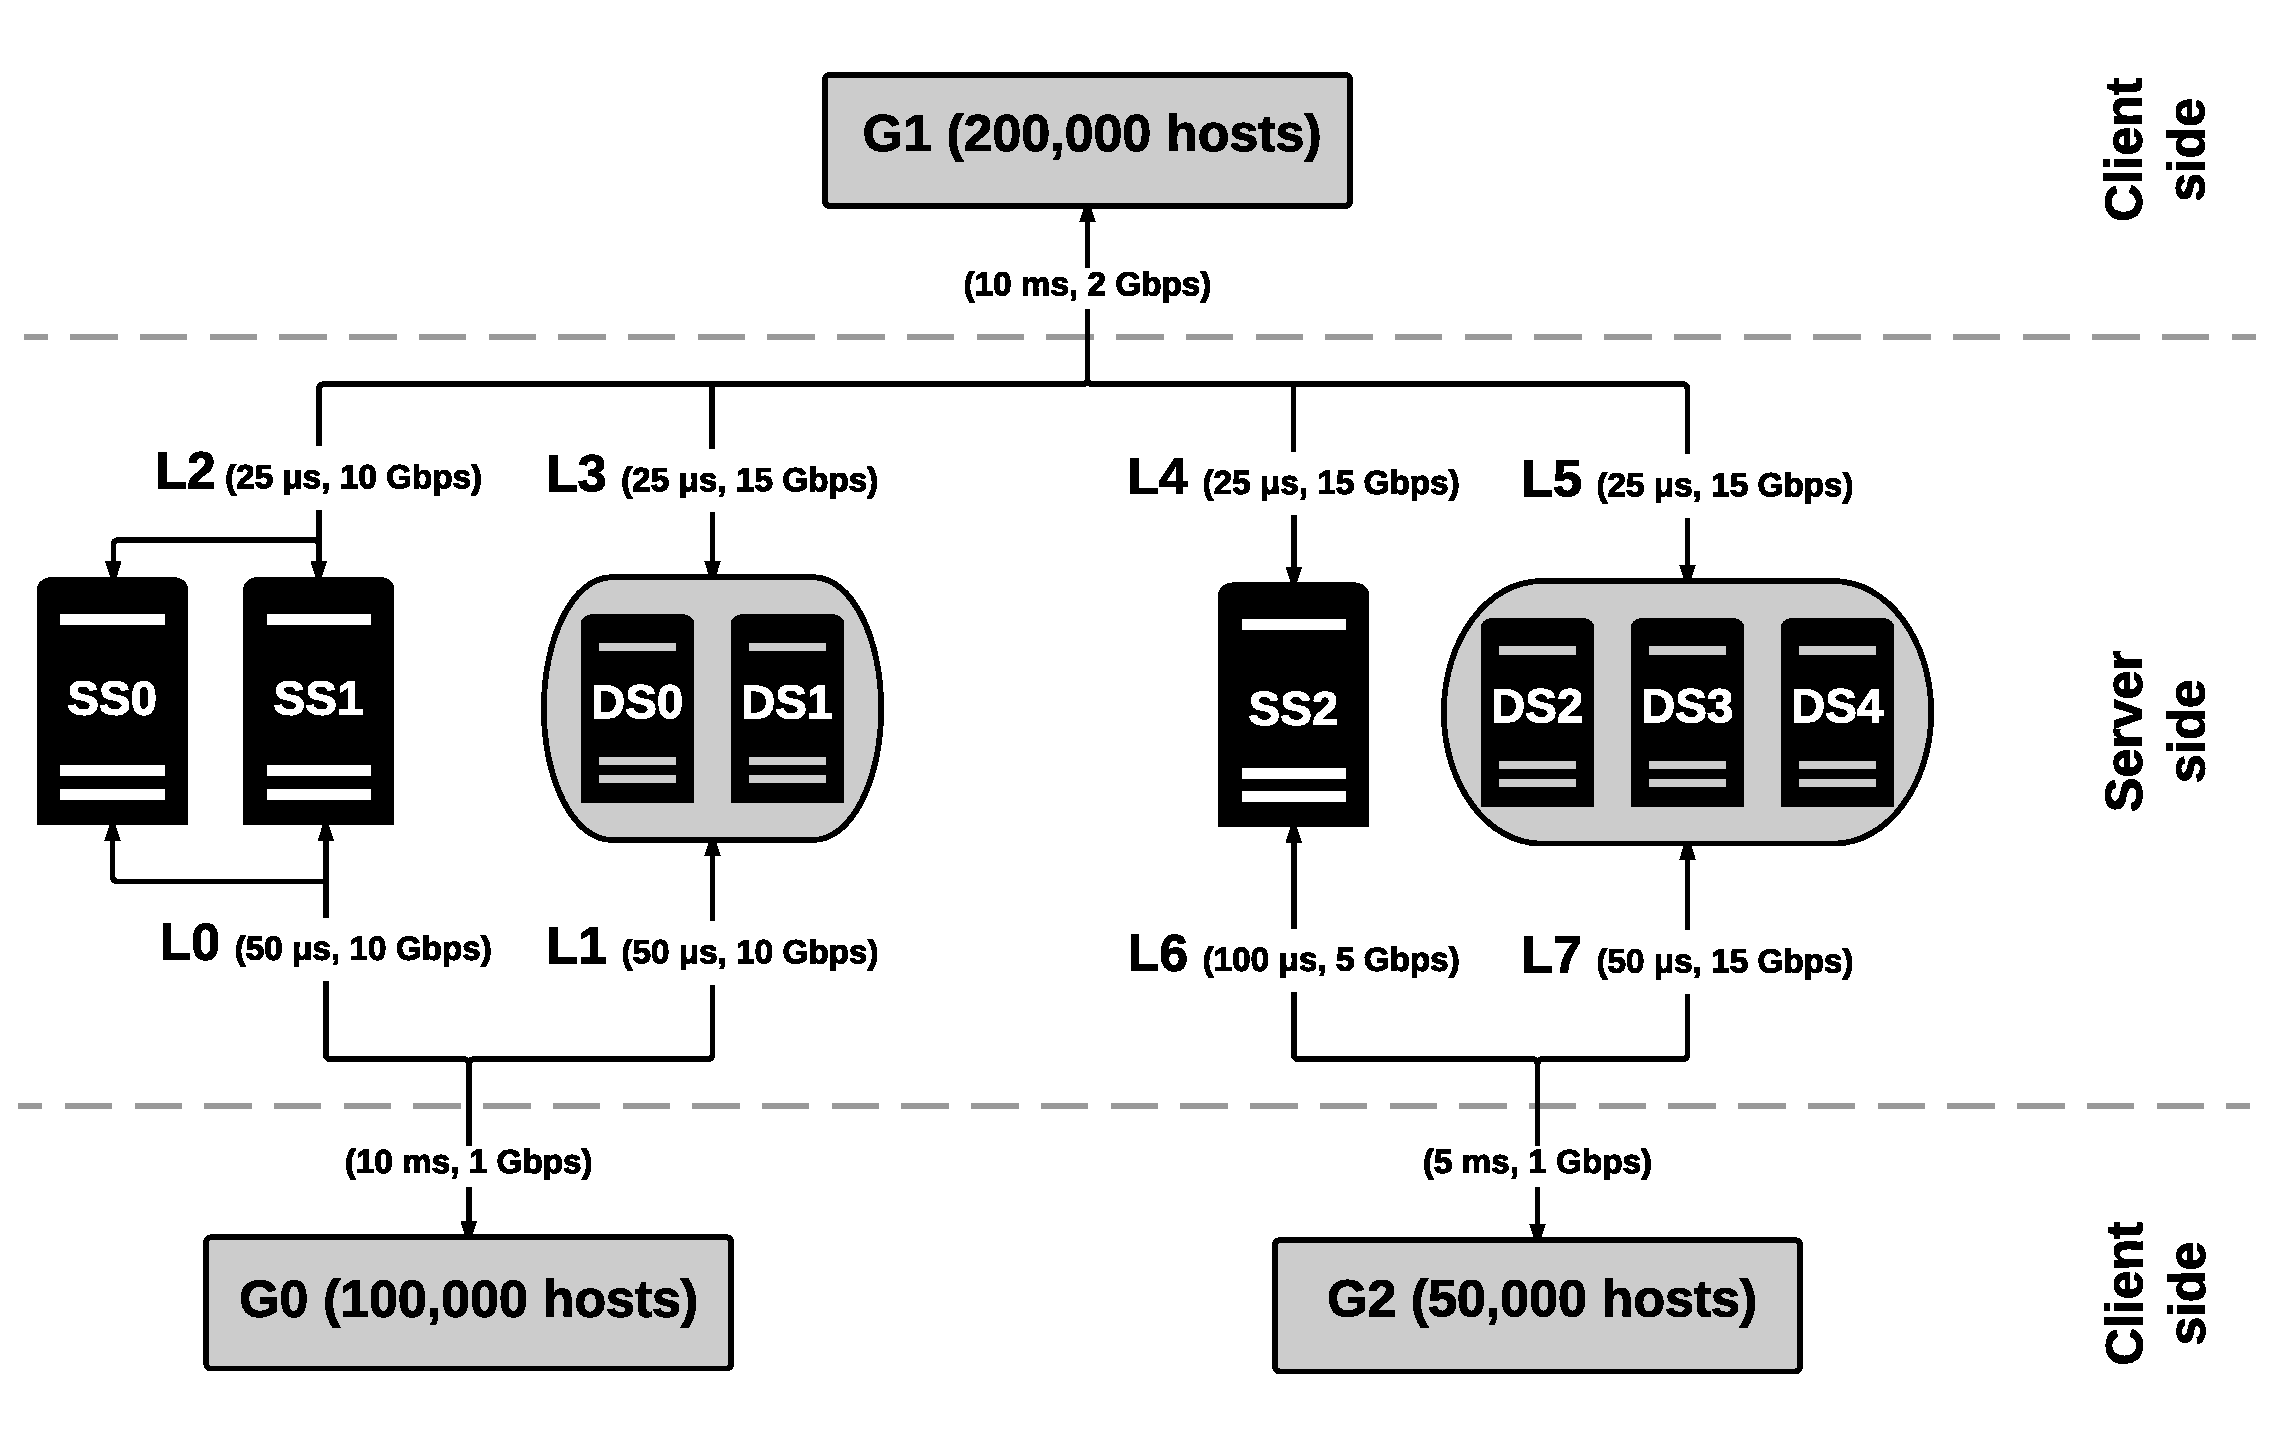
\includegraphics[width=13.5cm]{figures/interaction}
    \caption{Simulator platform example.}
    \label{fig:interaction}
\end{figure}

To create a simulation, \gls{comsimboinc} requires to specify all the parameters described in Tables \ref{tab:project_parameters} and \ref{tab:vngroup_parameters} in the parameters.xml file (see Listing \ref{lis:parameters}). Users can define the power and availability of the volunteer hosts via either a traces file or distribution functions. For example, in the case of the SETI@home project, we have analyzed the 3,900,000 hosts that participate in this project. The CPU performance of the hosts can be modeled according to an exponential function, as shown Figure \ref{fig:exponential}, which has a mean of 5.871 Giga\acrshort{flops} per host.

\begin{figure}[htbp] 
	\begin{subfigure}{0.5\textwidth}
		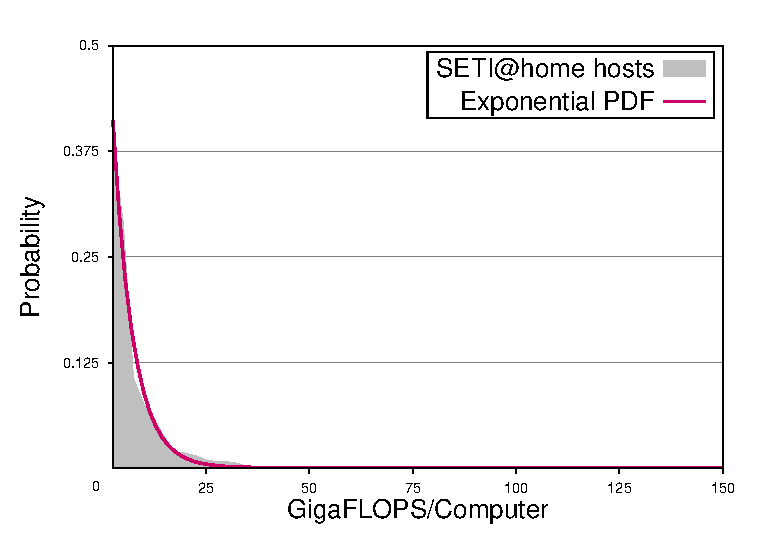
\includegraphics[width=\linewidth]{figures/density}
		\captionsetup{width=.9\textwidth}
		\caption{Probability density function of SETI@home hosts power.} 
		\label{fig:pdf}
	\end{subfigure}
	\hspace*{\fill} % separation between the subfigures
	\begin{subfigure}{0.5\textwidth}
		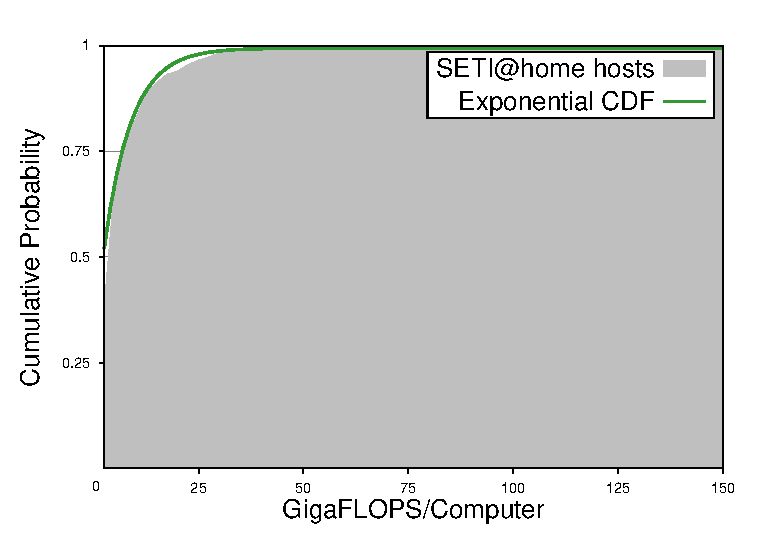
\includegraphics[width=\linewidth]{figures/distribution}
		\captionsetup{width=.9\textwidth}
		\caption{Cumulative distribution function of SETI@home hosts power.} 
		\label{fig:cdf}
	\end{subfigure}
	\caption{CPU performance modeling for SETI@home hosts.}
	\label{fig:exponential}
\end{figure}


Our software first processes the \gls{xml} file, creating the necessary deployment and platform files for subsequent simulations. In  \gls{comsimboinc}, all this is transparent to the user. The user only has to specify all the parameters of the simulation in the \gls{xml} file (Listing \ref{lis:parameters}), and run the generator script using the following command:

\vspace{0.6cm}

\begin{lstlisting}[language=bash]
  $ ./generator
\end{lstlisting}

\vspace{0.6cm}

The above command generates the platform and deployment files. The platform file contemplates all the necessary elements in the simulation: hosts, clusters, links, etc. The deployment file indicates the processes that should be created during the simulation. In addition, the generator script also compiles all source files needed for the simulation and generates the executable file. Finally, to run the simulation you just need to run the execution script:

\vspace{0.6cm}

\begin{lstlisting}[language=bash]
  $ ./execute
\end{lstlisting}

\vspace{0.6cm}

The execution results are composed by multiple statistical results (see Listings \ref{lis:output}): the execution time, the memory usage of the simulator, the load of the \gls{scheduling} and data servers, the total number of work requests received in the \gls{scheduling} servers, the job statistics (number of jobs created, sent, received, analyzed, success, fail, too late, etc), the credit granted to the clients, the number of \acrshort{flops}, the average power of the volunteer nodes, and the percentage of time the volunteer nodes were available during the simulation.

\clearpage

    \lstset{
    language=xml,
    morekeywords={Server, Client, side},
    tabsize=3,
    frame=lines,
    label=code:sample,
    frame=shadowbox,
    rulesepcolor=\color{gray},
    xleftmargin=20pt,
    framexleftmargin=15pt,
    numbers=left,
    numberstyle=\tiny,
    numbersep=5pt,
    breaklines=true,
    showstringspaces=false,
    basicstyle=\footnotesize,
    captionpos=b,
    caption=parameters.xml file filled with the parameters of the example.,
    label=lis:parameters}
    
    \lstinputlisting{figures/parameters.xml}
    
\clearpage

    \lstset{
    %language=xml,
    morekeywords={PROJECT1, PROJECT2},
    tabsize=3,
    frame=lines,
    label=code:sample,
    frame=shadowbox,
    rulesepcolor=\color{gray},
    xleftmargin=20pt,
    framexleftmargin=15pt,
    numbers=left,
    numberstyle=\tiny,
    numbersep=5pt,
    breaklines=true,
    showstringspaces=false,
    basicstyle=\footnotesize,
    captionpos=b,
    caption=Simulation execution results.,
    label=lis:output}
    
    \lstinputlisting{figures/output}
    
\end{appendices}